\documentclass{article}

\usepackage{graphicx} % Required for inserting images
\graphicspath{ {./images/} }
\usepackage{subcaption}

\usepackage{biblatex}
\addbibresource{references.bib}

\usepackage{csquotes}

\usepackage{tikz}
\usetikzlibrary{arrows,intersections,calc}

\usepackage{pgfmath}

\usepackage{listings}
\usepackage{color}

\DeclareMathSymbol{*}{\mathbin}{symbols}{"01}

\definecolor{dkgreen}{rgb}{0,0.6,0}
\definecolor{gray}{rgb}{0.5,0.5,0.5}
\definecolor{mauve}{rgb}{0.58,0,0.82}

\lstset{frame=tb,
  language=[5.2]Lua,
  aboveskip=3mm,
  belowskip=3mm,
  showstringspaces=false,
  columns=flexible,
  basicstyle={\small\ttfamily},
  numbers=none,
  numberstyle=\tiny\color{dkgreen},
  keywordstyle=\color{blue},
  commentstyle=\color{gray},
  stringstyle=\color{mauve},
  breaklines=true,
  breakatwhitespace=true,
  tabsize=3
}

\renewcommand{\abstractname}{Executive Summary}

\title{A three-dimensional rail shooter in PICO-8}
\author{Harry Jackson}
\date{September 2025}

\begin{document}
\maketitle

\begin{abstract}
The rail shooter was one of the earliest attempts to bring video
games into the third-dimension - first through the use of pseudo-3D
scaling effects, and later through the use of real-time polygonal graphics.

This project seeks to explore this category of interactive software through a
modern implementation incorportating polygonal rendering for PICO-8 - a
``fantasy console'' which replicates the computational and data constraints of
historical system hardware on which developers typically eschewed polygonal
rendering for simpler 2D effects.
\end{abstract}

\section*{Acknowledgements}

\tableofcontents

\section{Introduction, aims, and objectives}
[To be outlined and written after composition of rest of main body]


\section{Background and context}

\subsection{The rail shooter}
\subsubsection*{Historical outline}
Give broad overview of significance of rail shooters in the development of approaches
to 3D game design and chart their development with a focus on:
\begin{itemize}
   \item\textit{Space Harrier} and the 2D Super Scaler approach;
   \item\textit{Star Fox} as an exemplar for 16-bit polygonal 3D with
   cartridge storage limitations;
   \item\textit{Panzer Dragoon} as a 32-bit polygonal 3D game on optical media;
   \item and \textit{Rez} as a mature rail shooter with continued life in VR and
   ongoing aesthetic significance.
\end{itemize}

\begin{figure}[h]
\begin{subfigure}{.5\textwidth}
  \centering
  \includegraphics[width=.8\linewidth]{spaceharrier}
  \caption{\textit{Space Harrier} (1985)}
  \label{fig:sfig1}
\end{subfigure}
\begin{subfigure}{.5\textwidth}
  \centering
  \includegraphics[width=.8\linewidth]{placeholder}
  \caption{\textit{Star Fox} (1993)}
  \label{fig:sfig2}
\end{subfigure}
\begin{subfigure}{.5\textwidth}
  \centering
  \includegraphics[width=.8\linewidth]{panzerdragoon}
  \caption{\textit{Panzer Dragoon} (1995)}
  \label{fig:sfig3}
\end{subfigure}
\begin{subfigure}{.5\textwidth}
  \centering
  \includegraphics[width=.8\linewidth]{rez}
  \caption{\textit{Rez Infinite} (2016)}
  \label{fig:sfig4}
\end{subfigure}
\caption{the development of the rail shooter over time}
\label{fig:history}
\end{figure}

\subsubsection*{Gameplay taxonomy}
% Describe the basic structure of a 3D rail shooter with reference to the above examples,
% outlining their various approaches to core gameplay elements like enemy design, player
% movement, shooting and targetting, significant action set-pieces, and their use of
% fixed perspective or a malleable 3D camera.

Rail shooters have a relatively straightforward gameplay structure, in which players are
automatically carried forward along a fixed path - within which they exercise a fairly
limited range of motion along their relative x-axis and y-axis, and within which they
shoot enemies, and avoid both environmental obstacles and incoming enemy fire. In early instances,
the player moves in a straight line with limited freedom to veer (without gameplay consequence),
while later entries in the genre guided players through more complex spatial compositions incorportating
curves and varied levels of elevation.

Player movement typically doubles up as player aiming too - in early iterations of the genre like
\textit{Space Harrier} and \textit{Star Fox}, movement is tied directly to the player's aim in a
linear fashion, and in later polygonal titles the player directly controls the player's targetting
reticle with player model movement following in an indirect fashion. This differs from modern 3D
game input systems in which player movement and player aiming are controlled independently via dual 
analogue control - this sequence of games were largely developed in tandem with the rise of 3D console
gaming, and largely fell out of fashion before dual analogue input became ubiquitous following the
2000 launch of Sony's PlayStation 2.

% investigate camera controls in PD Orta, PD Remake, and Rez Infinite...

Later games in the cycle did contain rudimentary camera controls, however, with \textit{Panzer Dragoon}
allowing players to rotate the camera in 90 degree chunks using the Sega Saturn's shoulder inputs.
Players were able to see the location of off-camera enemies via a low fidelity radar in the heads up
display, requiring strategic decision making about which of four directions to shoot from.

% Discuss boss set pieces - eg multisprite enemies in Space Harrier, ship in Dragoon, sphere in Rez
\subsubsection*{Genre pitfalls}
Evidence common criticisms of 3D rail shooters as ``glorified technical demos'' with
limited room for gameplay innovation and discuss their waning significance in
commercial game design - with appropriate counter-examples of cult following for
balance.

\subsection{PICO-8}
\subsubsection*{Introduction to PICO-8}
% Discuss ethos of PICO-8 as a ``fantasy console'' and outline its technical
% specification - emphasis on compute power, memory limitations, screen resolution,
% player inputs, and token limits - and indicate some of the implications of these
% constraints on project scope.

... PICO-8 preamble ...

The system is built around the following key constraints\cite{white}:

\begin{itemize}
   \item a 128x128 pixel display
   \item a fixed palette of 16 colours
   \item execution of four million virtual instructions per second
   \item a sheet of 128 8x8 sprites
\end{itemize}

\subsubsection*{PICO-8 as prototyping tool}
Discuss benefits of using PICO-8 as a tool for rapid creation and iteration of
game prototypes, compare and contrast to full 3D engines like Unity, Godot and Unreal,
describe suitability given fixed time constraints of an individual summer
project, and point to games successfully prototyped in PICO-8 (most notably
\textit{Celeste}).

\subsubsection*{Sprite-scaling functionality}
% Discuss PICO-8's given functionality for sprite drawing and scaling and explain how
% these would facilitate development of a low-fidelity game utilising a pseudo-3D
% Super Scaler approach.
One specific advantage of using PICO-8 for this project, in addition to its general
advantages as a prototyping tool, is in-built support not only for drawing sprites
from a sheet but also for dynamically scaling sprites - the core rendering technique
that underlies the early Super Scaler games outlined in the previous section.

In addition to the standard sprite drawing call spr() - which is ideally suited to
typical 2D games in which sprites are drawn at a constant size - PICO-8 also offers
an sspr() function that allows the programmer to dynamically scale and stretch sprites.
This, wrapped in functionality to project points in 3D space to points on a 2D screen,
allows the sort of sprite scaling that can simulate depth in 3D space among
multiple 2D sprite assets.

\subsubsection*{Extensibility of 2D primatives for 3D}
% Discuss \textit{Star Fox} as exemplar polygonal rail shooter built within similar
% constraints and make critical comparison between PICO-8 platform specification and
% the Super Nintendo with on-cartridge Super FX graphics chip.
One ambition of this project, however, is to go a step beyond sprite scaling effects
and also introduce a limited degree of polygonal rendering - following the example of
Argonaut Software's 1993 Super Nintendo title \textit{Star Fox}, which leveraged bespoke
hardware to drive polygon rendering which is beyond PICO-8 only in scale.

% Discuss extensibility of PICO-8's functions for drawing primitives (eg rectfill and line)
% for triangle rasterisation and polygonal rendering.
Since, at root, polygonal rendering only requires the ability to draw triangles onto a
screen, PICO-8 can therefore perform the requisite functions if given primitive shape calls such
as line() and rectfill() are appropriately extended to draw filled shapes between three points.

\subsubsection*{3D experimentation in PICO-8}
Broad overview of existing experimentation with polygonal 3D in PICO-8 with a
focus on \textit{PICO-Fox} as closest analogue. 

Discuss exposed limitations of approach - particularly heavy cost of geometry data
for 3D models, and limitations imposed on design by use of polygonal enemies as
standard (ie minimum size constraint forced by low readability of small 3D models
on a coarse pixel grid).

\subsubsection*{Mitigation strategies for constraints}
Discuss apparent mitigation stategies to work effectively with PICO-8 in light of
the known constraints of the system. Emphasis on:
\begin{itemize}
   \item aggressive use of OOP to eliminate code dupication and preserve token count;
   \item use of standard 30Hz display mode rather than higher-refresh 60Hz mode, to
   trivially double frame budget when drawing and manipulating 3D models;
   \item a blended 2D/3D approach that reserves polygonal rendering for the player
   sprite and for boss encounters, and allows the flexibility and low cost of
   sprite-based gameplay throughout the rest of the core gameplay loop;
   \item possible growth into a ``multicart'' game, in violation of a basic intended
   constraint of the system, as a last resort to deal with token limits.
\end{itemize}


\section{Implementation I: Prototyping}

\subsection{Paper prototyping, software prototyping, and 3D rendering test}
The prototyping phase of the project began with three pieces of work along two tracks: firstly,
a paper prototype concretising the core gameplay loop, in which the player moves forward through
space and encounters enemies, and a software implementation of that paper prototype in PICO-8; and
secondly, initial technical work confirming the potential of PICO-8 for polygonal rendering and
allowing me to start getting to grips with the basic ideas behind real-time rendering in general.
\subsubsection*{Basic player actions using primatives}
Referring back to the gameplay taxonomy conducted in the background section, explain
how the most significant user actions were distilled down to fit a six-input
gamepad. Showcase how this was modelled using a flat paper prototype and outline
how this was translated into a software prototype using primitive shapes to model
the player and randomly spawned enemies, with movement and interactions being
directly translated into screen-space.

Highlight issues already identified at this early stage of prototyping - such as
player model blocking, the relationship between the player reticle and the destination
of projectiles in hypothecated 3D space, the need for limitations on enemy
target locking, and the need for game objects to have a meaningful existence in 3D
space.

\begin{figure}[h]
\begin{subfigure}{.5\textwidth}
  \centering
  \includegraphics[width=.8\linewidth]{placeholder}
  \caption{paper prototype}
  \label{fig:pfig1}
\end{subfigure}
\begin{subfigure}{.5\textwidth}
  \centering
  \includegraphics[width=.8\linewidth]{prototype2d}
  \caption{initial software prototype}
  \label{fig:pfig2}
\end{subfigure}
\caption{early prototyping}
\label{fig:gameprototype}
\end{figure}

\subsubsection*{Simple 3D renderer with model scaling and rotations}
Describe the contruction of a simple 3D renderer to prove suitability of PICO-8 for
the proposed project. Expose and discuss my implementation of triangle rasterisation
in PICO-8 and briefly explain the benefits of decomposing 3D shapes into triangles
rather than quads. Discuss related issues in polygonal rendering such as triangle
sorting and backface culling.

Showcase the results of the ``sanity test'', in which multiple
cubes are drawn to the screen progressively in order to understand the relative
computational cost of tracking and drawing 3D geometry in PICO-8 and the feasibility
of real-time polygonal rendering given system constraints and my existing quality
of implementation.

\begin{figure}[h]
\begin{subfigure}{.5\textwidth}
  \centering
  \includegraphics[width=.8\linewidth]{placeholder}
  \caption{single cube render}
  \label{fig:3dfig1}
\end{subfigure}
\begin{subfigure}{.5\textwidth}
  \centering
  \includegraphics[width=.8\linewidth]{test3d}
  \caption{multi-cube sanity check}
  \label{fig:3dfig2}
\end{subfigure}
\caption{early prototyping}
\label{fig:3dprototype}
\end{figure}

\begin{figure}[h]
\begin{center}
\begin{tabular}{r|c c c c c c c c c c}
     Cubes drawn & 0 & 1 & 2 & 3 & 4 & 5 & 6 & 7 & 8 & 9 \\
     \hline
     CPU utilisation & .37 & .39 & .41 & .43 & .46 & .47 & .49 & .50 & .52 & .53
\end{tabular}
\end{center}
\caption{CPU load sanity testing results}
\label{fig:3dtest}
\end{figure}

\subsection{3D conversion of software prototype}

While the initial software prototype served a useful purpose in allowing me to get comfortable
with core mechanics of the game, and in getting me to begin thinking about significant design
decisions that needed to be made, its origins in a flat paper prototype also led to key technical
implimentation issues being elided - namely the proper handling of depth and perspective necessary
to really deliver on the initial idea of the project.

As such, the initial software prototype was built on in the next phase of development and refactored
such that objects carried proper three-dimensional positions in world space, and were drawn in a
properly scaled and perspective correct way instead of having movement in depth simply faked through
rudimentary arbitrary re-scaling.

\begin{figure}[h]
    \centering
    \includegraphics[width=.8\textwidth]{explosion}
    \caption{final software prototype}
    \label{fig:particles}
\end{figure}

\subsubsection*{Graphical effects with 2D sprites and particles}
Describe the implementation of 2D sprites to replace primitive shapes used in earlier
iterations of the prototype. Discuss the design considerations that led to the
adoption of easily identifiable flying saucer and drone designs. Discuss simple
graphical effects used to eg light up flying saucer lights, or spin rotors of
enemy drones. Explain implementation of enemy destruction effects - namely the
implementation of a simple particle system over the bed of an explosion animation
efficiently faked by a combination of progressive scaling and random flipping of a
non-symmetrical sprite.

\subsubsection*{Perspective-correct 3D projection and scaling}
% Discuss the application of 3D point projection to the corners of 2D sprite objects
% to achieve perspective correct drawing and scaling of 2D elements using PICO-8's sspr
% function. Highlight use of small camera movements (spatial displacement in x and y)
% aligned to player sprite movement to heighten illusion of depth along the z-axis.
One of the key changes introduced in this 3D software prototype was the creation of accurate
depth among enemy units, created by correctly projecting sprite objects onto the screen using
newly introduced \textit{z}-coordinate values.

In order to accurately project a point from 3D space onto a screen, you must... \cite{gambetta}

TO DO: EXPLAIN GENERIC POINT PROJECTION EQUATION - LAW OF SIMILAR TRIANGLES ETC

\begin{figure}[h]
\begin{subfigure}{.45\textwidth}
   \centering
   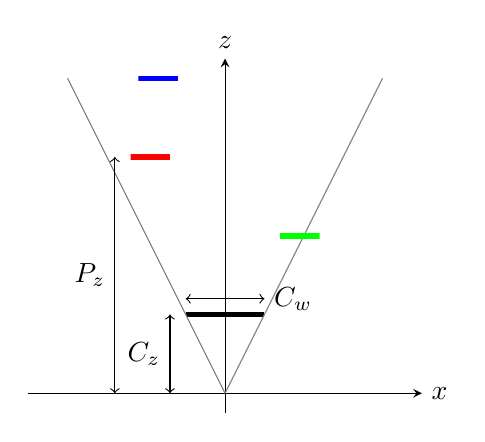
\begin{tikzpicture}
      [scale = 1,
      axis/.style={-stealth},
      dot/.style= {
         draw,
         fill = black,
         circle,
         inner sep = 0pt,
         minimum size = 4pt
      },
      point/.style= {
         draw,
         fill = black,
         circle,
         inner sep = 0pt,
         minimum size = 2pt
      }]
      
      \draw[axis] (-2.5, 0) -- (2.5, 0) node[right] {$x$};
      \draw[axis] (0, -0.25) -- (0, 4.25) node[above] {$z$};

      \draw[line width = 2] (-0.5, 1) -- (0.5, 1);
      \draw[draw = gray] (0, 0) -- (-2, 4);
      \draw[draw = gray] (0, 0) -- (2, 4);
      \draw[<->] (-0.7, 0) -- node[left] {$C_z$} (-0.7, 1);
      \draw[<->] (-1.4, 0) -- node[left] {$P_z$} (-1.4, 3);
      \draw[<->] (-0.5, 1.2) -- (0.5, 1.2) node[right] {$C_w$};

      \draw[line width = 2, draw = blue] (-1.1, 4) rectangle (-0.6, 4);
      \draw[line width = 2, draw = red] (-1.2, 3) rectangle (-0.7, 3);
      \draw[line width = 2, draw = green] (0.7, 2) rectangle (1.2, 2);

   \end{tikzpicture}
   \caption{top orthographic view}
   \label{fig:rotfig1}
\end{subfigure}\hfill
\begin{subfigure}{.45\textwidth}
   \centering
   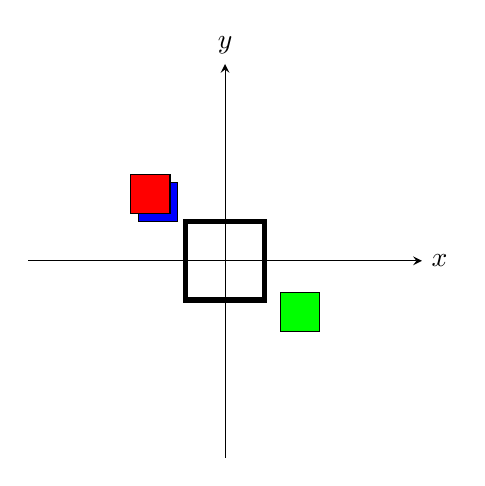
\begin{tikzpicture}
      [scale = 1,
      axis/.style={-stealth},
      dot/.style= {
         draw,
         fill = black,
         circle,
         inner sep = 0pt,
         minimum size = 4pt
      },
      point/.style= {
         draw,
         fill = black,
         circle,
         inner sep = 0pt,
         minimum size = 2pt
      }]
      
      \draw[axis] (-2.5, 0) -- (2.5, 0) node[right] {$x$};
      \draw[axis] (0, -2.5) -- (0, 2.5) node[above] {$y$};

      \draw[fill = blue] (-1.1, 1) rectangle (-0.6, 0.5);
      \draw[fill = red] (-1.2, 1.1) rectangle (-0.7, 0.6);
      \draw[fill = green] (0.7, -0.4) rectangle (1.2, -0.9);
      \draw[line width = 2] (-0.5, -0.5) rectangle (0.5, 0.5);

   \end{tikzpicture}
   \caption{front orthographic view}
   \label{fig:rotfig1}
\end{subfigure}\hfill
\begin{subfigure}{1\textwidth}
   \centering
   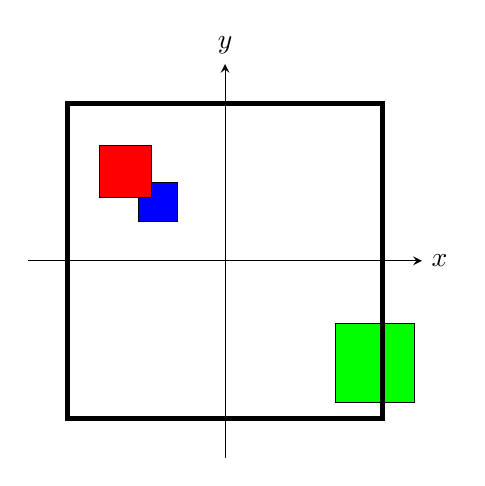
\begin{tikzpicture}
      [scale = 4,
      axis/.style={-stealth},
      dot/.style= {
         draw,
         fill = black,
         circle,
         inner sep = 0pt,
         minimum size = 4pt
      },
      point/.style= {
         draw,
         fill = black,
         circle,
         inner sep = 0pt,
         minimum size = 2pt
      }]
      \draw[axis] (-0.625, 0) -- (0.625, 0) node[right] {$x$};
      \draw[axis] (0, -0.625) -- (0, 0.625) node[above] {$y$};

      \draw[fill = blue] (-0.275, 0.25) rectangle (-0.15, 0.125);
      \draw[fill = red] (-0.4, 0.367) rectangle (-0.233, 0.2);
      \draw[fill = green] (0.35, -0.2) rectangle (0.6, -0.45);

      \draw[line width = 2] (0.5, 0.5) rectangle (-0.5, -0.5);


   \end{tikzpicture}
   \caption{perspective-correct projection of sprite objects onto screen}
   \label{fig:rotfig2}
\end{subfigure}\hfill
\caption{projection of a sprite objects in 3D space onto a canvas}
\label{fig:projection}
\end{figure}

This operation is implemented in the code using a single function that takes a three-component vector -
representing the \textit{x}, \textit{y}, and \textit{z} coordinates of a vertex in space - and projects them
onto a screen of width and height 1, centred around (0, 0) and located one unit along the \textit{z}-axis.

This positioning along \textit{z} and the use of a 1 by 1 screen simplifies the math required by reducing the
need for extraneous divisions and multiplications by arbitrary values, since any number divided or multiplied 
by 1 is unchanged - allowing us to cancel out variables in the projection equation as seen in
figure \ref{fig:equationsimpleproject}.

\begin{figure}[h]
   \begin{equation}
      C_x = \frac{P_x} {P_z} * C_w
   \end{equation}
   \begin{equation}
      C_y = \frac{P_y} {P_z} * C_h
   \end{equation}
   \caption{simplified projection equations}
   \label{fig:equationsimpleproject}
\end{figure}

Once the position of the vertex has been projected onto the screen in world space, it is then converted to
screen space by multiplication (by 128 - the pixel width and height of the screen in PICO-8) and displaced
appropriately by the approximate mid-point of the screen at pixel (64, 64).

This function is called twice for each sprite drawn, finding the position of the top-left and bottom-right
corners of its face and then drawing the sprite using PICO-8's in-built scaled sprite function sspr().

While the example illustrated in figure \ref{fig:projection} highlights the use of this function
to project the extreme corners of 2D sprites onto a screen, the same method is also used by the
program to project the three vertices of triangles onto screen space too - allowing the rendering of
polygonal shapes such as the player ship and the icosahedral boss enemy shell.

In the implementation highlighted in figure \ref{fig:codeproject} from the software prototype, displacements
in the \textit{x} and \textit{y} axes was added to represent relative motion of the camera - although this
effect was later removed from the final version of the game, since it tended to make the
gameplay harder to reason about spatially.

\begin{figure}[h]
   \begin{lstlisting}
   project_vert = function(vect3)

      return 64 + (((vect3[1] - camera.x) / vect3[3]) * 128), 64 - (((vect3[2] - camera.y) / vect3[3]) * 128)

   end
   \end{lstlisting}
   \caption{vertex projection function}
   \label{fig:codeproject}
\end{figure}

\subsubsection*{Real-time 3D collisions}
Discuss implementation of cuboid bounding volumes to test for collisions, using
height, width, and depth data paired if three-dimensional positions to check for
intersection of volumes. Discuss the need for axis-alignment to significantly
simplify calculations, and the design implications of this with regard to rotational
symmetry of objects depicted (ie disc-shaped saucers, and spherical projectiles)

\begin{figure}[h]
    \centering
    \includegraphics[width=.8\textwidth]{placeholder}
    \caption{collision of axis aligned cuboid bounding volumes}
    \label{fig:collision}
\end{figure}

\section{Implementation II: Full implementation}

Following extensive prototyping and the development of a functional software version that
implemented the core gameplay intended gameplay loop and incorporated both
perspective-correct sprite projection and polygonal rendering, it was time to start work on
the final implementation - starting with a properly designed software architecture and object
hierarchy that built on the lessons of early prototyping and properly ordered the software in
a rational, DRY, and polymorphic way.

In addition to a significant ground-up reworking of the second software prototype, development
also began on the end-game boss - featuring a more interactive polygonal element - and associated
problems with 3D geometry. This phase of the project also, ultimately, saw the project shift toward
a multicart design following a late encounter with PICO-8 token limits.

\subsection{Settled software architecture and object hierarchy}
Discuss the software architecture and walk through the significant parts of the
class diagram that was drafted at the end of software prototyping. Explain how the
design was informed by prototyping and broader game systems architecture reading.
Describe how game flow is controlled within the architecture. Descibe how game object
subclassing of sprite objects and polygonal objects facilitates the blended
2D/3D rendering approach outlined earlier in a polymorphic way. 

\subsection{Transition to multi-cart design}
Discuss late impact of token limit. Discuss decision to eschew imposed limitation of
PICO-8 and convert game to a multi-cart project. Discuss benefits of approach, including
introduction of straightforward game start/game over/restart logic based on storage of
pertinent persistent data and use of cart reloading. 

\subsection{The core game loop}
Describe the core gameplay loop and give a comprehensive tour of the update and draw
functions in main.lua that execute it, explaining the rationale for event and draw
sequencing. Discuss the z-sort implementation in draw, comparing to alternative sorting
algortithms, and describe how polymorphic class design enables heterogeneous elements
to be drawn together in the correct depth ordering.

\begin{figure}[h]
    \centering
    \includegraphics[width=.8\textwidth]{final3d}
    \caption{final software}
    \label{fig:3dfinal}
\end{figure}

\subsubsection*{The update loop}
Discuss gameworld object.

Outline update process of gameworld: character health check and possible exit to Game Over screen,
management of particular gameplay wave including generation of a new wave if necessary, followed by
an update of the existing or new wave, player update including inputs, followed finally by management
of game scenery, bullets, and various pick-up items.

Discuss the use of multicarting to control game menus, reset game state, and transition to boss mode
if the given wave target is reached.

Discuss the operations involved in the wave class - including selection of wave type, and how various
types of wave operate at initialisation and over the first 300 ticks of gameplay to generate enemies
with bespoke synchronised movement patterns.

Discuss the update operations of individual enemies including bullet collision checks, movement, and
timed firing. Discuss consequence of bullet collision, and creation of explosion objects - referring back
to prior section outlining the implementation of the explosion animation and particle effect.

Discuss player input scheme with particular reference to lock-on system.

Discuss scenery, bullet, and pick-up management. Justify timing of bullet update and outline alternative
approaches \cite{nystrom}.
\subsubsection*{The draw loop}
Discuss the initial drawing of a flat surface using rectfill() and its population by scrolling scenery.
Discuss the design decisions behind the use of trees, rocks, and clouds and their ability to be easily
rotated without jarring consequence. Discuss positioning of scenery outside the effective range of
play, and why this makes it appropriate to draw static scenery first.

Discuss the use of the z-sort algorithm to correctly order sprites and polygonal objects
for correct ordering by depth. 

Refer to earlier 3D projection discussion and discuss how this is used as the foundation for
spriteobject level draw calls that use object-level sprite-sheet data.

Discuss the use of pal() calls to simulate lights and rotary blades in the saucer and drone
enemies.

Discuss the use of backface culling for the player ship and the decision to draw backfaces
within the boss, allowing for the use of a hollow ``shell'' shape to enhance gameplay.

Discuss the use of recoloured sprites and semi-random sprite flipping to draw player thrusters
with a dynamic quality.

Discuss the in-game HUD. Trace its development from the initial software prototype, its brief
abandonment, and its reintroduction following user testing feedback about the failure of players
to engage with more traditional HUD elements on the borders of the display.

\subsection{Boss mode}

\begin{figure}[h]
\begin{subfigure}{.5\textwidth}
  \centering
  \includegraphics[width=.8\linewidth]{boss1}
  \caption{boss mode approach}
  \label{fig:bossfig1}
\end{subfigure}
\begin{subfigure}{.5\textwidth}
  \centering
  \includegraphics[width=.8\linewidth]{placeholder}
  \caption{boss mode gameplay}
  \label{fig:bossfig2}
\end{subfigure}
\caption{boss mode}
\label{fig:boss}
\end{figure}

\subsection{Some technical topics}

\subsubsection*{Camera rotations in 3D space}
Discuss the implementation of camera rotations around a point in 3D space for the
creation of a ``boss mode'' which involves strafing around a polygonal enemy. Highlight
the implications of this change on the position and orientation of the player model,
which can no longer exist naively in a 2D plane facing along the z-axis but which
must now be able to exist in a rotational relationship to a focal point in the map,
shared with the camera. Discuss the relationship between in-frame player movement,
the implied field of view of a 1x1 canvas at single unit distance from pinhole, and
camera rotation around a point. Discuss the per-object rotations required to execute
such camera movements, density of spawned scenery, and concerns around computational
load.

\begin{figure}[h]
\begin{subfigure}{.45\textwidth}
   \centering
   \begin{tikzpicture}
      [scale = 2,
      axis/.style={-stealth},
      dot/.style= {
         draw,
         fill = black,
         circle,
         inner sep = 0pt,
         minimum size = 4pt
      },
      point/.style= {
         draw,
         fill = black,
         circle,
         inner sep = 0pt,
         minimum size = 2pt
      }]
      
      \draw[axis] (-1.25, 0) -- (1.25, 0) node[right] {$x$};
      \draw[axis] (0, -1.5) -- (0, 1.5) node[above] {$z$};

      \draw (0.5, 0.5) node[dot, label = {above:$r$}] {};
      \draw [black, ->] (0.5, 0.5) -- (0, 0);

      \draw (-0.3, 0.6) node[point, label = {above:$o_1$}] {};
      \draw [gray, ->] (-0.3, 0.6) -- (-0.8, 0.1);
      \draw (-0.8, 0.1) node[point, label = {above:$t_1$}] {};

      \draw (0.9, 0.2) node[point, label = {above:$o_2$}] {};
      \draw [gray, ->] (0.9, 0.2) -- (0.4, -0.3);
      \draw (0.4, -0.3) node[point, label = {above:$t_2$}] {};

      \draw (-0.4, -0.4) node[point, label = {above:$o_3$}] {};
      \draw [gray, ->] (-0.4, -0.4) -- (-0.9, -0.9);
      \draw (-0.9, -0.9) node[point, label = {above:$t_3$}] {};

   \end{tikzpicture}
   \caption{select point \textit{r} in 2D plane around which to rotate scene, and translate
   all objects \textit{o} by the inverse of its position vector to positions \textit{t}}
   \label{fig:rotfig1}
\end{subfigure}\hfill
\begin{subfigure}{.45\textwidth}
   \centering
   \begin{tikzpicture}
      [scale = 2,
      axis/.style={-stealth},
      dot/.style= {
         draw,
         fill = black,
         circle,
         inner sep = 0pt,
         minimum size = 4pt
      },
      point/.style= {
         draw,
         fill = black,
         circle,
         inner sep = 0pt,
         minimum size = 2pt
      }]
      \draw[axis] (-1.25, 0) -- (1.25, 0) node[right] {$x$};
      \draw[axis] (0, -1.5) -- (0, 1.5) node[above] {$z$};

      \draw (0.5, 0.5) node[dot, label = {above:$r$}] {};

      \coordinate (R) at (0.5, 0.5);

      \pgfmathsetmacro{\angle}{70}
      \pgfmathsetmacro{\tx}{-0.8}
      \pgfmathsetmacro{\ty}{0.1}
      \coordinate (t1) at (\tx, \ty);
      \pgfmathsetmacro{\rx}{\tx*cos(\angle) - \ty*sin(\angle)}
      \pgfmathsetmacro{\ry}{\tx*sin(\angle) + \ty*cos(\angle)}
      \pgfmathsetmacro{\radius}{sqrt((\tx * \tx) + (\ty * \ty))}
      \coordinate (r1) at (\rx,\ry);
      \draw (t1) node[point, label = {above:$t_1$}] {};
      \draw (r1) node[point] {};
      \begin{scope}
         \clip (-1, \ty) rectangle (0, \ry);
         \draw[densely dotted] circle(\radius);
      \end{scope}
      \draw [gray, ->] (r1) -- ($(r1)+(R)$);
      \draw ($(r1)+(R)$) node[point, label = {above:$p_1$}] {};

      \pgfmathsetmacro{\tx}{0.4}
      \pgfmathsetmacro{\ty}{-0.3}
      \coordinate (t2) at (\tx, \ty);
      \pgfmathsetmacro{\rx}{\tx*cos(\angle) - \ty*sin(\angle)}
      \pgfmathsetmacro{\ry}{\tx*sin(\angle) + \ty*cos(\angle)}
      \pgfmathsetmacro{\radius}{sqrt((\tx * \tx) + (\ty * \ty))}
      \coordinate (r2) at (\rx,\ry);
      \draw (t2) node[point, label = {above:$t_2$}] {};
      \draw (r2) node[point] {};
      \begin{scope}
         \clip (1, \ty) rectangle (0, \ry);
         \draw[densely dotted] circle(\radius);
      \end{scope}
      \draw [gray, ->] (r2) -- ($(r2)+(R)$);
      \draw ($(r2)+(R)$) node[point, label = {above:$p_2$}] {};

      \pgfmathsetmacro{\tx}{-0.9}
      \pgfmathsetmacro{\ty}{-0.9}
      \coordinate (t3) at (\tx, \ty);
      \pgfmathsetmacro{\rx}{\tx*cos(\angle) - \ty*sin(\angle)}
      \pgfmathsetmacro{\ry}{\tx*sin(\angle) + \ty*cos(\angle)}
      \pgfmathsetmacro{\radius}{sqrt((\tx * \tx) + (\ty * \ty))}
      \coordinate (r3) at (\rx,\ry);
      \draw (t3) node[point, label = {above:$t_3$}] {};
      \draw (r3) node[point] {};
      \begin{scope}
         \clip (t3) rectangle (\rx, -1.5);
         \draw[densely dotted] circle(\radius);
      \end{scope}
      \draw [gray, ->] (r3) -- ($(r3)+(R)$);
      \draw ($(r3)+(R)$) node[point, label = {above:$p_3$}] {};

   \end{tikzpicture}
   \caption{rotate translated points \textit{t} around (0, 0) and translate them again by positive
   position vector of chosen point of rotation to find final position \textit{p}}
   \label{fig:rotfig2}
\end{subfigure}\hfill
\caption{\textit{y}-axis rotation of a scene around an arbitrary point in 3D space}
\label{fig:rotation}
\end{figure}

\subsubsection*{Ray-triangle collision with the Möller–Trumbore algorithm}
Discuss the need for more complex ray-triangle intersection computations to effectively
test for collisions around the boss enemy, since the intended design requires per-face
collision detection on a regular icosahedron whose faces cannot be satisfactorily
split into non-overlapping cuboid bounding volumes that adequately approximate
collisions.

\section{Results}
\subsection{Think-aloud testing feedback}
Discuss feedback gathered by think-aloud testing sessions, and highlight adaptations
to the software intended to answer constructive criticisms. Possible subjects of
discussion:
\begin{itemize}
   \item implementation of on-player HUD to answer lack of player attention on vital
   gameplay statistics, ie remaining life and state of lock-on targetting;
   \item redesign of pick-up sprites to better differentiate power-ups from
   damage-inducing projectiles;
   \item introduction of narrative splash screen to justify on-screen action, which
   was seen as random and unexplained.
\end{itemize}
Also discuss positive feedback gathered during sessions, such as satisfaction
with the game controls, hit detection, and overall aesthetic of the game, and comfort
with depth perception despite the low-resolution pixel grid.
\subsection{Formal NASA-TLX testing}
I also subjected my programme to one round of quantitative testing to investigate the
relative contributions of enemy speed and enemy fire rate to overall difficulty - as
measured by task load.

This was done through the use of the widely used and validated NASA-TLX survey on which...

TO DO: GENERAL EXPLANATION OF NASA-TLX

Participants were asked to play three builds of the game - a control build, in which enemy
ships behaved in a ``normal'' way, a rapid fire build in which enemy ships move at a standard
speed but fire more quickly, and a rapid movement build in which the rate of fire is the same
as in the control but the ships move faster.

TO DO: CALCULATE RESULTS OF NASA-TLX SURVEYS TAKEN ON 11/08


\section{Evaluation}
\subsection{Pitfalls of paper prototyping for 3D projects}
Discuss issues raised by developing initial software prototype from a paper prototype
- with emphasis on inate tendancy of paper prototyping to flatten images to a surface,
mask issues relating to depth-in-space, and discourage serious thinking about the
relationship between world-space and screen-space in projects like this.
\subsection{Artificial limits imposed by featly to platform ethos}
Discuss late move to multicart approach and the creative envelope it opened - too late
in the project. Discuss attempts to remain within arbitrary token limit for much of the
project and speculate about additional game modes that could have been introduced hardware
a multicart approach been taken sooner (including both alternative boss designs, more
data-intensive 3D ideas, and variations on the core gameplay loop)
\subsection{Unavoidable limitations imposed by PICO-8}
Discuss issues caused by coarseness of PICO-8 pixel grid and difficulties caused by
limited fixed colour palette of PICO-8, and its impact on effective shading of polygonal
models. Discuss use of music and sound in \textit{Rez} and limitations imposed by PICO-8's
low-fi sound system - with equal recognition of creative limitations of developer.


\section{Further work}
\subsection{Additional mode development}

\begin{figure}[h]
\begin{subfigure}{.45\textwidth}
  \centering
  \includegraphics[width=.8\linewidth]{placeholder}
  \caption{an example of side-on action in \textit{Rez Infinite}}
  \label{fig:sideways}
\end{subfigure}\hfill
\begin{subfigure}{.45\textwidth}
  \centering
  \includegraphics[width=.8\linewidth]{placeholder}
  \caption{an example of shmup gameplay, entered into seamlessly from a traditional rail-shooter section, in \textit{Split Fiction}}
  \label{fig:shmup}
\end{subfigure}\hfill
\caption{boss mode}
\label{fig:additionalmodes}
\end{figure}

\subsubsection*{Sideways chase}
Discuss possibility of side-on scrolling action as seen in \textit{Panzer Dragoon} and \textit{Rez}.
Discuss feasibility of implementation given multi-cart approach and existence of functionality to
rotate camera around an arbitrary point.

IF TIME: BUILD RUDIMENTARY PROTOTYPE

\subsubsection*{Shmup mode}
Brief explanation of shmups. Discuss affinity between rail shooters and shmups. Describe rail section
of \textit{Split Fiction} and seamless transition between game modes. Discuss feasibility given
existing codebase.

\subsection{Change of technology}
\subsubsection*{Fully-featured game engine: Unreal, Unity, Godot}
\subsubsection*{Minimal game development library: raylib}
Discuss possible alternative benefits of developing using a minimal library like raylib,
which offers similarly freeform low-overhead development to PICO-8 without extraneous
constraints. Note flexibility of the library and ability to use bindings in a range of
languages rather than just Lua or the specified scripting languages imposed by fully-featured
off-the-shelf game engines.


\section{Conclusion}
[To be outlined and written after composition of rest of main body]

\printbibliography

\end{document}